\chapter{Preliminares}\label{chapter:REV-LL}

Este trabajo pretende implementar un sistema que resuelva instancias de VRP en cualquiera de sus variantes con el menor trabajo humano posible. En este capítulo se presentan los principales elementos de la investigación realizada para lograrlo.

Primeramente se comienza con una explicación general del problema de enrutamiento de vehículos (VRP) y algunas de sus variantes con la sección \ref{2-VRPintro}. Se explica cómo describir a partir de código una solución de VRP.

En \ref{2-Libr} se muestran las bibliotecas de clases existentes hasta el momento que pueden ser utilizadas para encontrar soluciones a problemas de VRP.

En \ref{2-Hector} se explica cómo crear un Árbol de vecindad a partir de una solución inicial y un criterio de vecindad. Este árbol es utilizado para obtener la cardinalidad de vecindades y generar soluciones.

En \ref{2-JJ} se expone el concepto de Grafo de evaluación y cómo es esto utilizado para evaluar soluciones de forma eficiente y automática.

En \ref{2-Heidy} se presenta un mecanismo para explorar vecindades de forma automática a partir de combinaciones de cualesquiera estrategias de exploración y selección.

Finalmente en \ref{2-Lisp} se describe brevemente algunas características y funcionalidades del lenguaje Common Lisp que resultaron especialmente útiles para el desarrollo del sistema.


%\newpage

\section{Problema de Enrutamiento de Vehículos}\label{2-VRPintro}
La primera referencia al VRP fue hecha por Dantzing y Ramser en \cite{Ramsin1959} en el año 1959. Se propone una formulación matemática, una aproximación algorítmica y se describe una aplicación real entregando gasolina a varias estaciones de servicio. 

En su versión más simple, VRP consta de una flota de vehículos que salen de un depósito y deben satisfacer las demandas de una serie de clientes. El objetivo es encontrar una distribución de caminos a asignar a los vehículos de forma que se optimice determinada métrica (tiempo, combustible, etc). Con más de 50 años de estudios se ha ramificado en una inmensa cantidad de variantes entre las que se pueden contar las siguientes:

\begin{itemize}
	\item CVRP - VRP con restricciones de capacidad. Cada vehículo tiene una capacidad que no debe ser excedida.
	\item VRPTW - VRP con ventanas de tiempo. Cada cliente posee un período de tiempo fijo durante el cual puede ser atendido.
	\item VRPPD - VRP con recogida y entrega. Los bienes deben ser entregados y recogidos en cantidades fijas.
	\item MDVRP - VRP con múltiples depósitos. Se cuenta con múltiples depósitos desde los que pueden salir los vehículos.
\end{itemize}

Esta es una familia de problemas NP-Duros\cite{TODO}, por lo las soluciones exactas no son factibles para instancias con muchas entradas (clientes). Para buscar aproximaciones a la solución se utilizan heurísticas y metaheurísticas. Se destaca la búsqueda local como metaheurística que ha dado muy buenos resultados encontrando óptimos \cite{TODO} y es la seleccionada en el presente trabajo como se explica en \ref{2-Local}. 

Para resolver un VRP es necesario definir qué se entiende por \textbf{solución}.

\subsection{Representación de soluciones del VRP}\label{2-Sol}
Las soluciones son representadas (en su versión más simple) como una serie de listas de clientes denominadas rutas.
Si se define a $P_1$ como un problema clásico (VRP en su versión mas simple) que consta de 6 clientes: $[c_1, c_2, c_3, c_4, c_5, c_6]$, entonces una solución $s_1$ se puede definir como:

\begin{equation}
	s_1 = [(c_2,c_3), (c_1,c_4,c_5), (c_6)]
\end{equation}

En $s_1$ se representa una solución con tres rutas. El vehículo perteneciente a la primera ($r_1$) ruta visita a $c_2$ y $c_3$, el vehículo de la segunda ruta ($r_2$) visita a $c_1$, $c_4$ y $c_5$ y el de la tercera ($r_3$) sólo visita a $c_6$. 

Encontrar la solución óptima exacta no es factible para instancias grandes. Para resolver VRP computacionalmente en un tiempo factible se utilizan metaheurísticas \cite{TODO}. Específicamente, el presente sistema utiliza Metaheurísticas de Búsqueda Local \cite{TODO}.

\subsection{Metaheurística de búsqueda local}\label{2-Local}
Los algoritmos basados en búsqeuda local son aquellos en que se define una solución inicial y a partir de determinado criterio de vecindad se busca la solución óptima iterando por los vecinos de la vecindad formada por dicho criterio. 

Por ejemplo, en VRP los criterios de vecindad consisten en conjuntos de movimientos de los elementos que conforman las rutas, ya sea dentro de una misma ruta o de unas hacia otras. A continuación se muestran algunos ejemplos de criterios de vecindad de VRP \cite{TODO}:

\begin{enumerate}
	\item Cambiar de posición a un cliente dentro de su ruta.
	\item Mover a un cliente de ruta.
	\item Intercambiar dos clientes de posición.
	\item Cambiar vehículo de ruta.
	\item intercambiar dos subrutas entre sí.
	\item invertir orden de una subruta (porción de una ruta).
\end{enumerate}

Los criterios de vecindad dependen también de la variante del problema sobre la que se trabaje. Por ejemplo, el criterio de \textbf{"Cambiar vehículo"} no tiene sentido para el problema $P_1$ pues en este todos los vehículos son iguales.

A los movimientos que conforman los criterios se les denomina operaciones de vecindad. Las operaciones pueden ser obtenidas a partir de un subconjunto de operaciones más simples a las que se denomina operaciones elementales. Entre las operaciones elementales se encuentran: \textbf{selección de ruta}, \textbf{selección de cliente} e \textbf{inserción de cliente} que comunmente se representan con los símbolos \textit{r}, \textit{a} y \textit{b} respectivamente. 

Por ejemplo \textit{intercambiar dos clientes de posición} es un criterio de vecindad conformado por las operaciones:

\begin{enumerate}
	\item Seleccionar ruta \textit{r1}.
	\item Seleccionar cliente \textbf{c1} de la ruta \textit{r1}.
	\item Seleccionar ruta \textit{r2}.
	\item Seleccionar cliente \textit{c2} de la ruta \textit{r2}
	\item Intercambiar clientes \textit{c1} y \textit{c2} de posición.
\end{enumerate}

Pero también por las operaciones:

\begin{enumerate}
	\item Seleccionar ruta \textit{r1}.
	\item Seleccionar cliente \textbf{c1} de la ruta \textit{r1}.
	\item Seleccionar ruta \textit{r2}.
	\item Seleccionar cliente \textit{c2} de la ruta \textit{r2}
	\item Insertar cliente \textit{c1} en la ruta \textit{r2} en la posición de \textit{c2}
	\item Insertar cliente \textit{c2} en la ruta \textit{r1} en la posición de \textit{c1}
\end{enumerate}


A partir de un criterio de vecindad y una solución inicial se pueden generar nuevas soluciones. El proceso de obtención y selección de nuevas soluciones se denomina exploración de la vecindad. La cardinalidad de una vecindad está dada por el número de vecinos que la forman. Mientras mayor la cardinalidad de la vecindad es más probable encontrar mejores soluciones \cite{TODO}, pero esto puede ser ineficiente computacionalmente \cite{TODO}. Por tanto, las estrategias (de exploración de vecinos y selección de mejoras) a seguir durante la exploración de una vecindad son un factor vital a tener en cuenta para la creación del sistema implementado en el presente trabajo y se explicarán en \ref{2-Hector} y \ref{2-Heidy}. Además, a la hora de comparar el costo entre dos soluciones es necesario evaluarlas, lo cual puede poseer también costo computacional alto. Para la evaluación de soluciones se tiene el Grafo de evaluación explicado en \ref{2-JJ}. 

Una buena herramienta para resolver problemas de VRP en la actualidad es la biblioteca OR-Tools (Google Optimization Tools)\cite{TODO}. Un software de código abierto útil para problemas de optimización combinatoria entre los que se encuentra el Problema de Enrutamiento. 

Un paso importante durante la exploración de una vecindad es la generación de los vecinos que conforman dicha vecindad. En el sistema implementado los vecinos se generan a partir de un Árbol de Vecindad.

\section{Árbol de vecindad}\label{2-Hector}
La exploración de vecindades puede ser ineficiente y difícil de programar. En \cite{Hector} se propone la representación de una vecindad mediante un árbol al que se denomina Árbol de Vecindad.

Todas las soluciones de una vecindad pueden ser obtenidas aplicando sobre la solución inicial el criterio de vecindad en cuestión de todas las formas posibles. A la asignación de valores (qué ruta se selecciona, qué índice tiene el cliente a seleccionar dentro de la ruta, etc) a los elementos que forman las operaciones de un criterio de vecindad se le llamará una instanciación de dicho criterio. Por ejemplo, dado el criterio \textbf{mover cliente} dado por las operaciones: 

\begin{itemize}
	\item Seleccionar ruta (r1).
	\item Seleccionar cliente (c1) de ruta (r1).
	\item Seleccionar ruta (r2).
	\item Insertar cliente (c1) en ruta (r2).
\end{itemize}

Un ejemplo de instanciación de este criterio sobre la solución $s_1$ se presenta como:

\begin{itemize}
	\item $r_1 = 1$ $\rightarrow$ $r_1$ es la ruta de la que el cliente $c_1$ es extraído.
	\item $c_1$ = 1 $\rightarrow$ $c_1$ es el primer cliente de la ruta.
	\item $r_2 = 2$ $\rightarrow$ $r_2$ es la ruta en la que el cliente $c_1$ será insertado.
	\item $c_1$ = 2 $\rightarrow$ $c_1$ es insertado en la posición 2 de la ruta seleccionada.
\end{itemize}

A cada vecino de un criterio se le puede hacer corresponder una instanciación del mismo y por tanto, encontrar la cardinalidad de una vecindad es similar a encontrar el número de instanciaciones posibles del criterio asociado.

Al computar la cardinalidad de una vecindad del VRP, se utiliza una estrategia recursiva que consiste en contar para una operación el número de secuencias de operaciones instanciadas que se pueden formar con el resto de las operaciones del criterio, así como combinar las mismas con las posibles instanciaciones de la operación actual. Lo que se propone en \cite{Hector} es utilizar dicha estrategia para almacenar toda la información necesaria para instanciar las operaciones que conforman la vecindad en una estructura arbórea que será llamada Árbol de Vecindad y que constituye una representación de la vecindad en cuestión mediante la que pueden ser generados todos los vecinos.

En la figura \ref{fig:neigh-tree} se muestra una representación del árbol de vecindad asociado al criterio \textbf{mover cliente} ($rarb$).

% TODO: \usepackage{graphicx} required
\begin{figure}
	\centering
	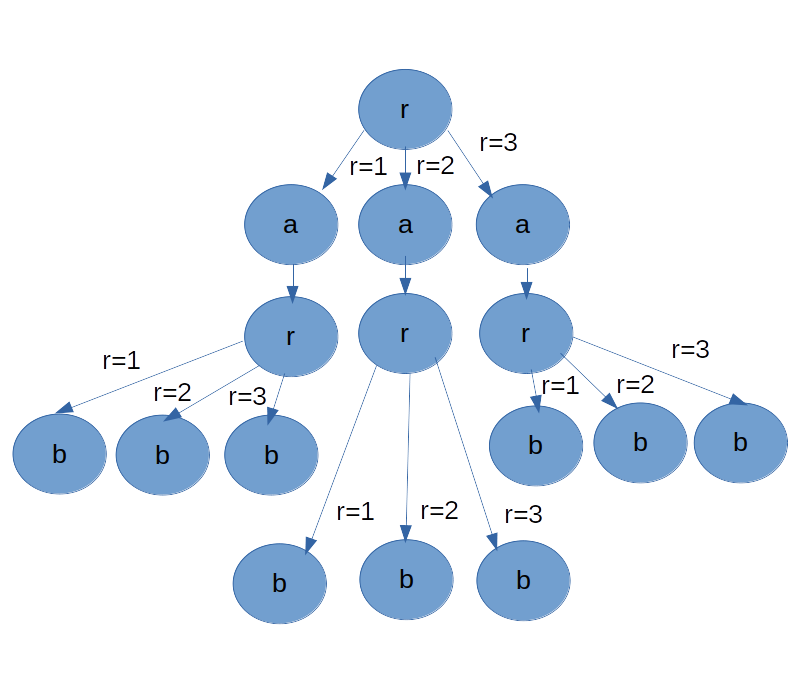
\includegraphics[width=0.9\linewidth]{Graphics/Neigh-Tree}
	\caption{Árbol de vecindad asociado a $rarb$}
	\label{fig:neigh-tree}
\end{figure}

Para obtener una instancia del criterio representado por un árbol y por tanto generar el vecino que se le corresponde basta con dar valores a (las operaciones representadas por) los nodos que conforman una rama del árbol. Por ejemplo, en el caso de la figura \ref{fig:neigh-tree} qué ruta o cliente seleccionar o dónde insertar un cliente

Cada conjunto de asignación de valores a los nodos de una rama se asocia a un índice $i$ con $1<=i<=k$ siendo $k$ la cardinalidad de la vecindad. Al indexar $i$ en el árbol, este genera una solución.  

Cada rama del árbol representa un conjunto de soluciones, por tanto, el conjunto de ramas representa una partición de la vecindad a la que está asociado dicho árbol. A los conjuntos hechos por esta partición se les denomina regiones y resultan útiles para encontrar características compartidas en grupos de vecindades. Por ejemplo, es conveniente analizar cuáles son las regiones con soluciones de menor costo para intensificar en estas la búsqueda de soluciones óptimas.

Luego de generadas las soluciones a partir del Árbol de Vecindad, es necesario conocer sus costos. Para esto se utiliza un Grafo de Evaluación.

\section{Grafo de Evaluación}\label{2-JJ}
Durante la exploración de las vecindades es generalmente necesario evaluar las soluciones que se van analizando (es posible, por ejemplo, querer contar los vecinos repetidos de una vecindad, en este caso no hay necesidad de evaluarlos). Ya sea para retornar inmediatamente una solución mejor a la inicial (estrategia de selección de primera mejora), para devolver la mejor solución (estrategia de selección de mejor vecino) o un vecino aleatorio entre todos los que mejoren la solución (estrategia de selección de mejor vecino aleatorio), en todos los casos hay que determinar el costo de las soluciones exploradas para analizar lo que es "mejor". Encontrar el costo de una solución es lo que se denomina como evaluar.

La evaluación de soluciones es potencialmente costosa. En el caso más simple de VRP se debe sumar las distancias entre cada cliente de cada ruta y el depósito. Agregar restricciones al problema implica análisis extra como la aplicación de penalizaciones a rutas con vehículos sobrecargados en el caso de CVRP \cite{TODO}.

El Grafo de Evaluación, propuesto por Jose Jorge Rodríguez en \ref{2-JJ}, permite evaluar soluciones vecinas a una solución inicial de forma eficiente ya que garantiza que sólo se recalculan los fragmentos de las nuevas soluciones en los que estas se diferencien de la solución inicial.

La estructura propuesta para evaluar una solución es una representación en forma de grafo de la evaluación dicha solución. Sus nodos están divididos en dos tipos: Nodos de alto nivel y nodos de bajo nivel. Los nodos de bajo nivel representan operaciones que reciben como entradas ciertos nodos de alto nivel y modifican con sus salidas otros nodos de alto nivel.

Por ejemplo, en la figura \ref{fig:eval-graph-1} se muestran los nodos de alto nivel del grafo que representa la solución: $s = [(c_1,c_2), (c_3,c_4)]$. Los nodos \textit{d} representan al depósito y el nodo $cost$ almacena el valor del costo total de la solución. Nótese que todas las rutas en el grafo comienzan y terminan con nodos depósito. 

\begin{figure}
	\centering
	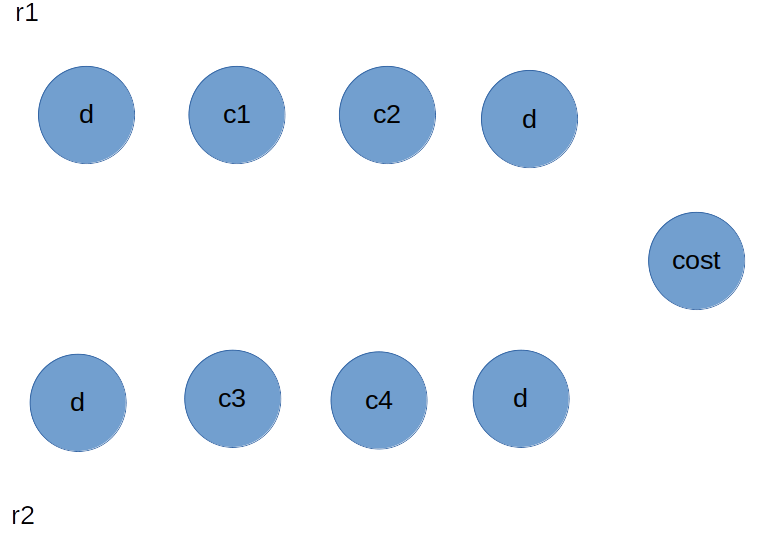
\includegraphics[width=0.9\linewidth]{Graphics/eval-graph-1}
	\caption{Nodos de alto nivel en un grafo de evaluación que representa la solución $s1$ de VRP clásico.}
	\label{fig:eval-graph-1}
\end{figure}

En \ref{fig:eval-graph-2} se muestra una representación del grafo completo para esta solución. Los nodos con símbolo de incremento son nodos de bajo nivel que toman como entrada dos nodos clientes (o depósito) y como salida adicionan al nodo de costo total la distancia entre ellos.

\begin{figure}
	\centering
	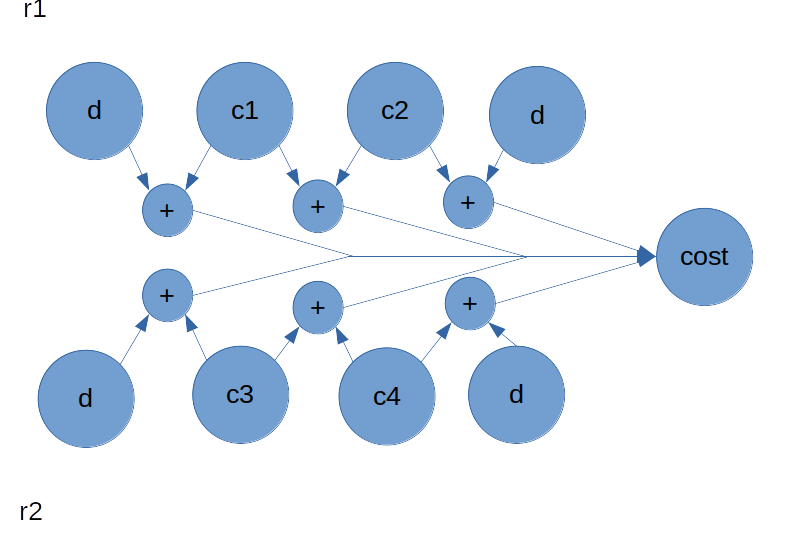
\includegraphics[width=0.9\linewidth]{Graphics/eval-graph-2}
	\caption{Grafo de evaluación que representa la solución $s1$ de VRP clásico.}
	\label{fig:eval-graph-2}
\end{figure}

En \ref{fig:eval-graph-3} se transforma el problema en CVRP utilizando la misma solución. En este caso se agregan los nodos de alto nivel $cap$ que tienen como valor inicial la capacidad del vehículo perteneciente a cada ruta. Los nodos de decremento reciben un cliente como entrada y, como salida, disminuyen la capacidad del vehículo en una cantidad igual a la demanda del cliente. Luego, los nodos $pen$ (también de bajo nivel) reciben como entrada los nodos de capacidad y, en caso de tener estos valor negativo, como salida penalizan el costo total de la solución.

\begin{figure}
	\centering
	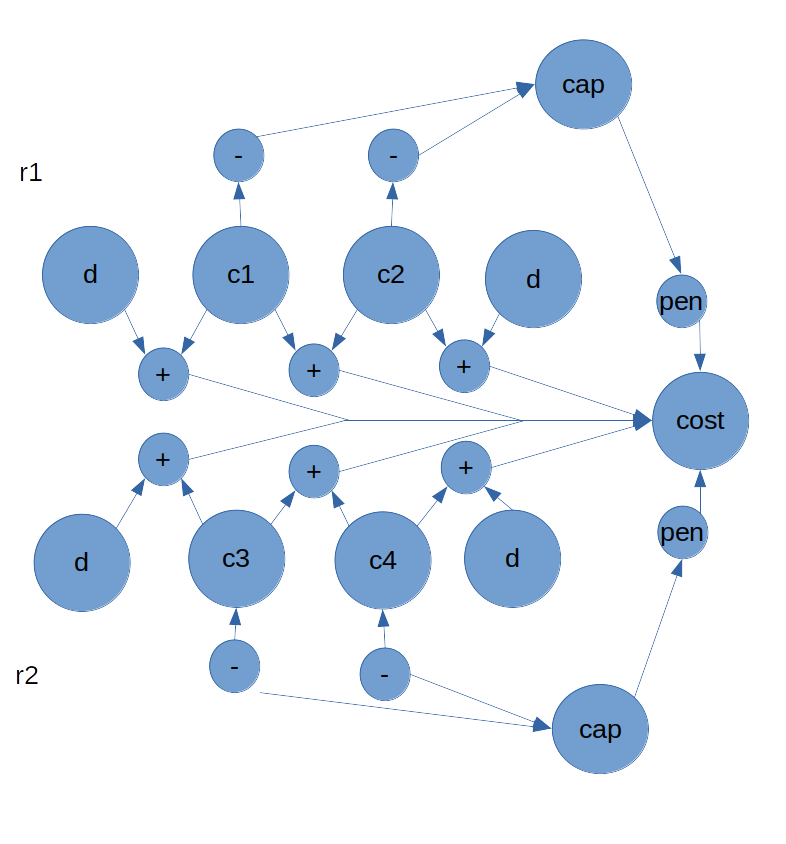
\includegraphics[width=0.9\linewidth]{Graphics/eval-graph-3}
	\caption{Grafo de evaluación que representa la solución $s1$ de VRP con restricciones de capacidad.}
	\label{fig:eval-graph-3}
\end{figure}

Todos los nodos de bajo nivel tienen asociado una función \textbf{evaluate} (para evaluar) y una función \textbf{undo} (para desevaluar) que son ejecutados cuando se agregan o remueven nodos de alto nivel. Por ejemplo, retirar un cliente $C1$ del grafo representado en \ref{fig:eval-graph-2} (VRP clásico) provoca que los dos nodos de incremento que utilizan dicho cliente como entrada se desevalúen y al mismo tiempo se crea un nuevo nodo incremento que recibe como entrada $d$ y $c2$. Luego, insertar a $c1$ al final de la ruta $r2$ implicaría desevaluar el nodo incremento que recibe como entrada a $c4$ y $d$ mientras se crean dos nodos incrementos nuevos, uno recibiendo de entrada a $c4$ y $c1$ mientras que el otro a $c1$ y $d$. El resultado de estas dos operaciones se muestra en \ref{fig:eval-graph-4} y es, precisamente, el grafo resultante de aplicar la siguiente instanciación del criterio $rarb$:

\begin{itemize}
	\item Seleccionar ruta (r1).
	\item Seleccionar cliente (c1) en ruta (r1).
	\item Seleccionar ruta (r2).
	\item Insertar cliente (c1) en posición (3) en ruta (r2).
\end{itemize}

Nótese que luego de aplicar los métodos \textbf{evaluate} y \textbf{undo} correspondientes el nodo $cost$ tiene almacenado el costo de la solución resultante luego de aplicar una instancia del criterio $rarb$. Para encontrar el costo de la nueva solución sólo fue necesario analizar y modificar los nodos en que el grafo de la solución nueva se diferencia con la solución anterior y no todo el grafo. En esto se basa la evaluación "eficiente" del Grafo de Evaluación.

\begin{figure}
	\centering
	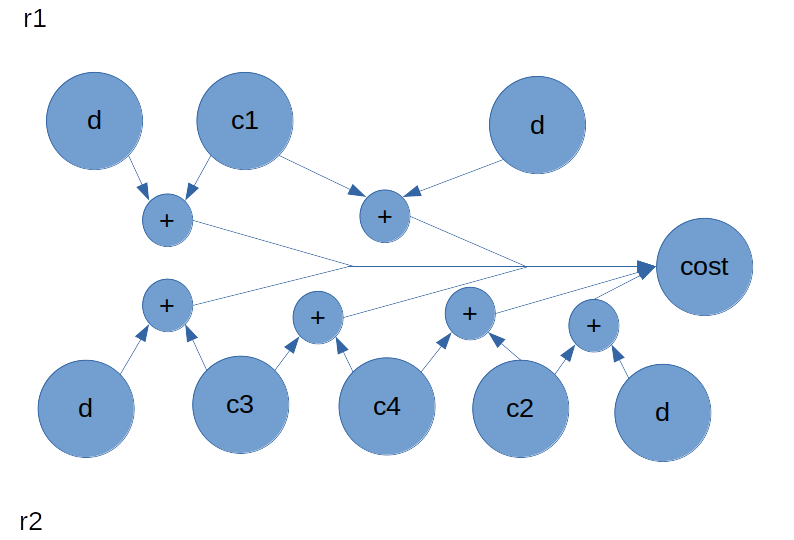
\includegraphics[width=0.9\linewidth]{Graphics/eval-graph-4}
	\caption{Grafo de evaluación que representa la solución $s1$ de VRP clásico luego de aplicada una instancia de $rarb$}
	\label{fig:eval-graph-4}
\end{figure}

Para construir el grafo que representa la solución inicial el usuario debe ingresar el códio de evaluación de esa primera solución. Luego, los costos el resto de las soluciones generadas son obtenidos al aplicar operaciones sobre el grafo inicializado.

Para explorar una vecindad a partir de un criterio es necesario (además de generar y evaluar soluciones) decidir e implementar estrategias de exploración y de selección. A partir de combinaciones de diferentes estrategias se pueden realizar exploraciones con distintos resultados.


\section{Combinación de estrategias de exploración y selección.}\label{2-Heidy}
En el proceso de exploración de una vecindad se parte de una solución inicial, se generan soluciones vecinas a esta (con el Árbol de vecindad) y se evalúan para comparar y obtener mejores soluciones (Grafo de Evaluación). Al explorar, deben también tenerse en cuenta problemas tales como vecindades con cardinalidades tan grandes que provoquen exploraciones ineficientes o el retorno de mínimos locales\cite{TODO}. Para una vecindad con muchas soluciones tal vez dé mejor resultado explorar no todos sus vecinos, sino una porción aleatoria de estos. Tal vez retornar siempre al mejor vecino de cada vecindad pueda provocar el encuentro de un mínimo local que se hubiera evitado seleccionando aleatoriamente cualquier solución que mejorara la inicial \cite{TODO}.

Al espectro de búsqueda de vecinos en una vecindad se le denomina estrategia de exploración. Algunos ejemplos son:

\begin{itemize}
	\item Exploración exhaustiva: Se analizan todos los vecinos que puedan ser generados.
	\item Exploración aleatoria: Se genera una cantidad fija de vecinos menor que la cardinalidad de la vecindad. La decisión de qué vecinos generar es aleatoria.
\end{itemize}

Además de decidir qué vecinos explorar, también es necesario decidir cuál retornar entre aquellos que mejoran la solución. A esta decisión se le denomina estrategia de selección. Se tiene como ejemplos:

\begin{itemize}
	\item Mejor vecino: Se retorna al mejor vecino entre todos aquellos analizados.
	\item Primera mejora: En el momento en que se encuentra un vecino mejor que el inicial, este es retornado.
	\item Mejora aleatoria: Se retorna un vecino aleatorio entre todos aquellos mejores que la solución inicial.
\end{itemize}

A partir de distintas combinaciones de estrategias de exploración y selección es posible realizar exploraciones distintas que obtengan diferentes resultados.

La propuesta de Heidy Abreu en \cite{Heidy} permite generar funciones de exploración fabricadas a partir de un criterio, una estrategia de selección y una de exploración. Las estrategias se definen como clases que se pasan como instancias a la función generadora (función que genera funciones de exploración). La función de exploraciñon resultante recibe el problema que se quiere resolver junto con una solución inicial, ejecuta la exploración y retorna una solución mejor en caso de existir dentro de la vecindad definida por el criterio. 

En el presente trabajo, el árbol de vecindad y el grafo de evaluación forman parte también de las funciones de exploración creadas. Un árbol de vecindad genera las soluciones y un grafo de evaluación se usa para evaluarlas. El grafo debe ser pasado como entrada también a la función de exploración.

La creación automática de funciones de exploración con distintas combinaciones de estrategias de exploración y selección se logra aprovechando sus características comunes y estructuras similares. El código generado en todas las funciones se reparte en cinco regiones que se  unen para generar una función completa. Las regiones y el tipo de código que pertenece a cada una se explicarán en \ref{2-blueprint}.

Para generar código crear funciones a partir de estrategias diferentes se utilizan características del lenguaje Common Lisp \cite{TODO} tales como la herencia múltiple y su sistema de objetos \cite{TODO}.

\section{Common Lisp y sus funcionalidades}\label{2-Lisp}
Common Lisp es un lenguaje de programación multi-paradigma (soporta una combinación de paradigmas de programación tales como la programación imperativa, funcional y orientada a objetos). Facilita el desarrollo de software evolutivo e incremental, con la compilación iterativa de programas eficientes en tiempo de ejecución.

El lenguaje acepta herencia múltiple. Esta característica permite crear jerarquías con clases que implementan funcionalidades de varias clases superiores. Por ejemplo, la clase que representa la estrategia de selección de mejor vecino (\textbf{best-improvement}) hereda de una clase que indica  retorno de mejor solución (\textbf{return-best-solution}) y de otra que indica el uso de un grafo de evaluación (\textbf{use-eval-graph}).

La herencia resulta especialmente útil para el presente trabajo cuando se combina con el sistema CLOS (Common Lisp Object System). Un mismo método puede tener numerosas implementaciones (especificaciones) que se ejecutan de acuerdo a los tipos de los parámetros proveídos como entradas. Además, también se ejecutan todas las especificaciones cuyos parámetros coincidan con los ancestros de los tipos de las entradas. Todas las especificaciones se combinan alrededor de un método primario conformando un único método con la unión de todos los códigos. El orden en que se combinan los métodos depende del orden de herencia y de los parámetros :before, :around y :after con que se definen.

Como ejemplo se tiene que para generar el código de la función de exploración para la estrategia de selección mejor vecino se une el código de métodos cuyo parámetro de \text{search-strategy} (estrategia de exploración) tenga tipo \textbf{best-improvement}, \textbf{return-best-solution}, \textbf{use-eval-graph} y cualquier otra clase que herede de alguna de estas. 

En el siguiente capítulo se explica cómo está orgainzado el sistema implementado, sus características y cómo fueron ensambladas sus piezas.



























